O método proposto segue um modelo híbrido para gerar objetos de aprendizagem por meio da agregação de artefatos multimídia em vídeos educacionais. Este método combina técnicas automáticas para geração de objetos multimídia com uma abordagem crowdsourcing para utilizar de forma eficiente as contribuições dos estudantes.

\begin{figure}[ht]
\centering
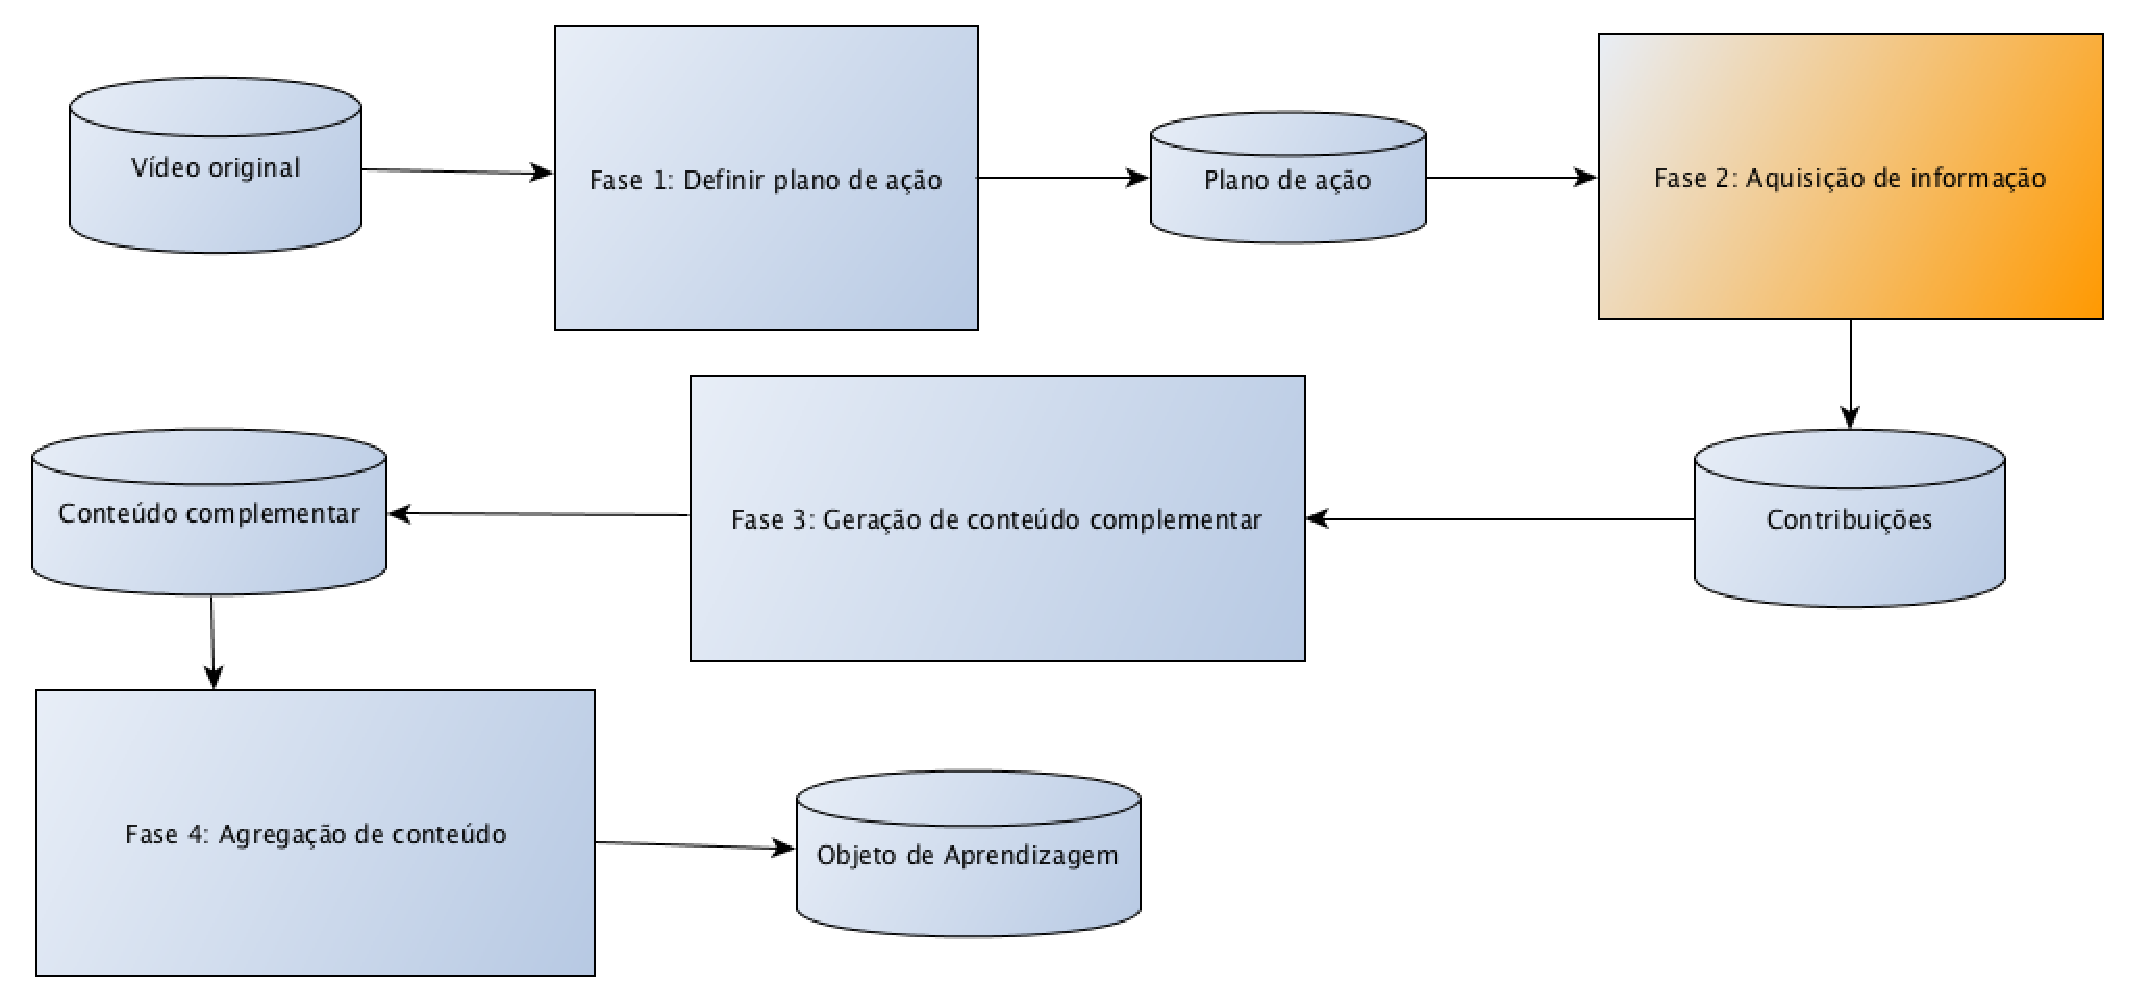
\includegraphics[width=.99\textwidth]{imagens/metodo/geral_oa.eps}
\caption{Visão geral do método}
\label{fig:metodo:geral}
\end{figure}


Conforme pode ser observado na Figura~\ref{fig:metodo:geral}, o método estabelece um processo para o enriquecimento do vídeo original, que resulta em um objeto de aprendizagem.

De forma resumida, o processo é realizado da seguinte maneira: inicialmente são definidas as características do objeto de aprendizagem a ser gerado, e a criação do plano de ação que deve ser seguido a fim de produzir o objeto de aprendizagem correto. Uma que o plano de ação está definido, tem inicio o processo crowdsourcing que utiliza as contribuições dos estudantes para determinar quais são as informações que devem ser utilizadas para gerar o conteúdo complementar. Após a coleta e processamento das contribuições, têm inicio a geração automática dos artefatos multimídia que serão agregados ao vídeo original. Por fim, após todos os artefatos estarem prontos, se faz o alinhamento deles sobre a linha do tempo do vídeo para que eles possam ser exibidos nos momentos corretos.










